\section{PLATOSim}
PLATOSim is a Simulator developed by the University Leuven which generates data as the PLATO mission will do, by simulating the whole acquisition process. The process aims to synthesize the satellite images as realisticly as possible by including all known noise sources and generating a numerically modelled imagette for each considered star. 
\newline
PLATOSim is planned to be a tool for the scientific comunity which is easily adaptable for other high-precision photometric space missions as well, therefore it is build very versatile and easy tweakable in its parameters. At the time beeing its main usage is by the different workgroups which develop software applications for the PLATO mission. PLATOSim is operational but stil in the process of testing and is adapted according to the needs of the different users from the aformentioned workgroups.
\newline
In this section the architecture and the mode of operation of the tool and all considered influence parameters are described.
\subsection{In- and Output}
In this section the in- and output of PLATOSim is discussed. 
\subsubsection{Output}
The goal of PLATOSim is the generation of the imagettes which are used to create the light curves of a star. Those imagettes are squared grayscale pictures centered around a star with a variable edge length. For the fast-cameras, which are used for the FGS position estimation imagettes with an edge length of 9 pixels are used. For every exposure there is a seperate imagette. All imagettes for a single star are stored in a hdf5 file. In figure \ref{fig:imagettes} three imagettes from three different stars are depicted. 

\begin{figure}[!htb]
\minipage{0.32\textwidth}
  
\includegraphics[width=\linewidth]{Imagette1.JPG}
\endminipage\hfill
\minipage{0.32\textwidth}
  
\includegraphics[width=\linewidth]{Imagette2.JPG}
\endminipage\hfill
\minipage{0.32\textwidth}%
  
\includegraphics[width=\linewidth]{Imagette3.JPG}
\endminipage
\centering
\caption{Output Imagettes from PLATOSim3}\label{fig:imagettes}
\end{figure}

To retrace the steps which let to the creation of the different help matrices as well as the subpixel map of the imagette and the corresponding psf are included too. Furthermore all information about the star, like its position in space and on the CCD, its ID number and its magnitude are stored in the hdf5 file.
\subsubsection{Input}
To create the desired data some information have to be given by the user of the simulator. The basis of the input is the star catalog which lists all stars, a simulation should be run for. This is a simple text--file which contains the right-ascension, the declination and the magnitude of every star in one line seperated by white spaces. Furthermore, there is an input--file where the user can configure the parameters of the simulation. There are possibilities to in- or exclude certain effects or noise sources and to alter numerical data like the orientation of the used telescope or of the CCD with respect to the pointing direction of the spacecraft. Some sources of disturbance need more direct input than random generated numbers, therefore files of the jitter movement and the thermo--elastic drift are present as well. The jitter--file includes the yaw, pitch and roll angles over which the axises of the spacecraft is rotated for a given time. Those data are stored as numbers, seperated by white spaces, in a text--file in which every line represents a measuring step.    
\subsection{Architecture}
PLATOSim3 aims to simulate the work of the PLATO satellite as close to reality as possible. Therefore the architecture of the program consists of 5 major parts to depict the spacecraft in its orbit and all the processes necessary for the data generation and one governing part, which controlls the information flow between them. Those parts are namely the platform, the telescope, the camera, the detector, the sky and the simulation. The main objective of each of those program parts is as follows:

\begin{itemize}
	\item platform -- stores information about the satellites movement e.g. jitter
	\item camera -- application of the point spread function
	\item detector -- administration of the different (sub-)pixel maps
	\item telescope -- provides information about the thermo-elastic drift
	\item sky -- includes data about the stars
	\item simulation -- organisation and flow control 
\end{itemize} 

\begin{figure}[h]
	\centering
	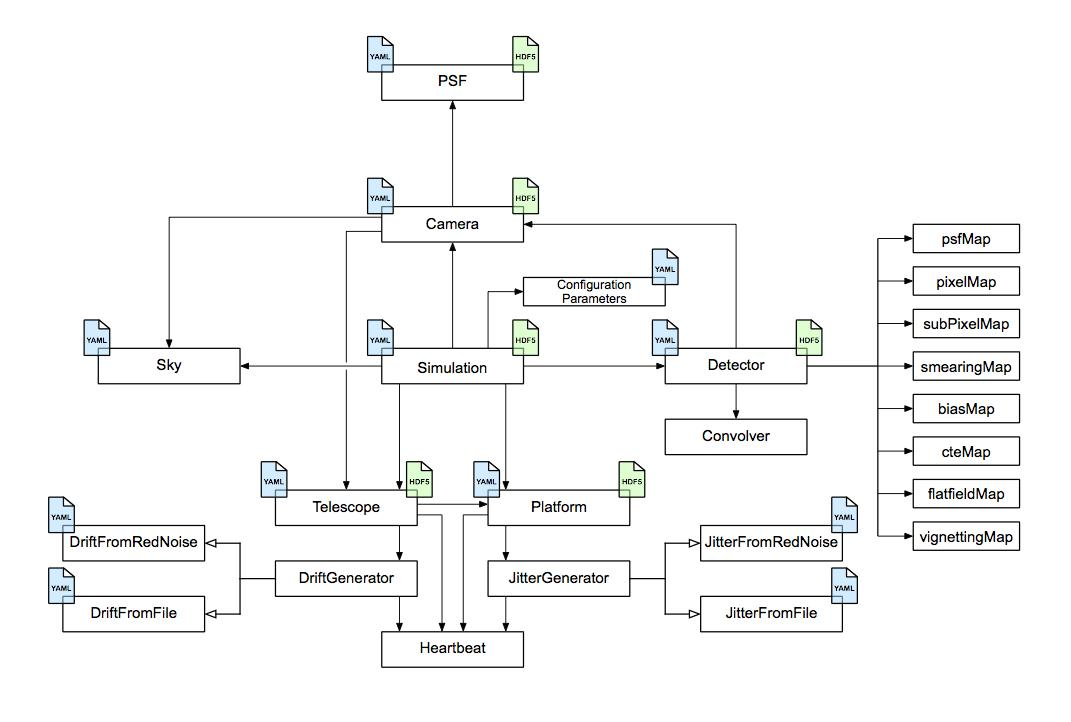
\includegraphics[width=\textwidth]{PLATOSim_design.jpg}
	\caption{PLATOSim process}
	\label{fig:mesh3}
\end{figure}

In this section the workflow of PLATOSIM will be presented along these program parts. First the managing simulation process is shown after which the details of the different simulation parts will be revealed.   
\subsection{Simulation Process}  
The working process of PLATOSim is shown in figure \ref{fig:mesh1}. In this section The single steps are shown and analysed for their relevance for the fine guidance system.

\begin{figure}[h]
\centering
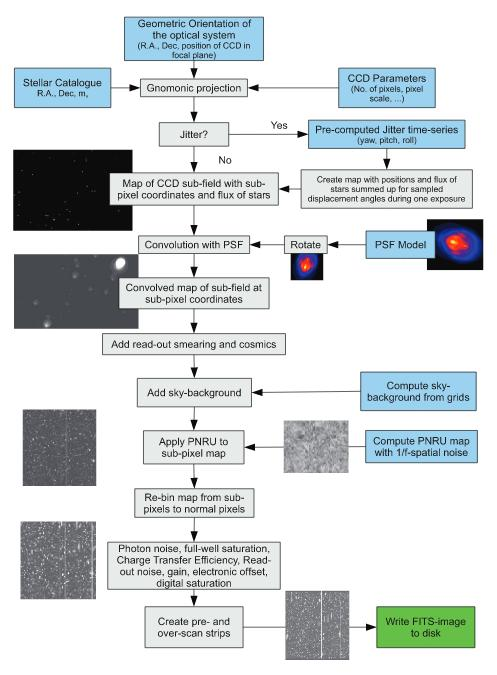
\includegraphics[width=\textwidth]{PLATOSim_Ablauf.jpg}
\caption{PLATOSim process}
\label{fig:mesh1}
\end{figure}

PLATOSim aims to generate only one imagette for one star with one exposure of the camera at the time. The whole CCD is generally not calculated because of the high memory consumption, which would be needed for such a task. Instead only the small section, where the light of the specific star falls on the CCD is simulated.
\newline
To correctly simulate motions and noise effects even the relatively small size (18 mycrometer) of the pixels is too large. Therefore it is necessary to subdivide each physical pixel in a number of subpixels to display intra-pixel sensitivities. The aforementioned imagette is enlarged in its dimensions depending on the number of subpixels the user wishes. All effects like the PSF or noise sources are applied on this subpixelmap, before it's rebinned again to the small imagette in the end. The more subpixels are used, the more accurate the result will be in theory.  However a larger subpixel map comes always at the price of longer processing times and more needed memory. 

\subsubsection{Geometry}
The first step is to determine where a star falls on which CCD of a camera. Therefore a few input data are required. The most important ones are the information about the currently 			relevant star and the orientation of the pointing axis of the satellite.

\subsection{Using PLATOSim for the FGS testing}
Whether PLATOSim3 is suitable for the testing of the FPS is dependant on mainly two things -- its speed and its precision in generating the output imagettes. The FGS of the PLATO mission has to be able to determine the position and orientation of the spacecraft from the output of the sensors in real time. Therefore the output of any simulator has to produce imagettes at least as fast as the fast cameras of PLATO would deliver them. The precision of PLATOSim3 is highly dependable on the correct mathematical representation of the effects the starlight causes on the CCD sensors. In the next subsections both aspects will be discussed.
\newline
To test the capabilities of PLATOSim3 a series of four simulations was conducted. The simulations were created using the following input parameters:
\begin{itemize}
	\item usage of the same catalog with 134 stars
	\item 1000 exposures of the detector
	\item gaussian PSF with 0.5 standard deviation
	\item no other noise source than jitter
	\item gradual increase of the number of subpixels used (128, 256, 512, 1024)
\end{itemize}
The goal of those simulations were the deduction of the influence of the number of subpixels on the quality of the position estimation with the FGS, as well as the measuring of the time needed to create a single output imagette. 
\newline
PLATOSim3 is a tool designed for a serial creation of imagettes for one star after another. However, to reduce the duration of a simulation (one simulation means in this context the generation of 1000 imagettes for all stars in the catalog) a computer cluster with 24 cores is used, which can conduct the simulation of 24 stars parallel, reducing the time of each simulation series to 5\% of its initial value. This greatly improves the possibilities to generate output but looses its usefullnes with higher numbers of subpixels. The problem is the convolution of the used psf with the created subpixel matrix for an imagette. Both matrices have the size of ~12000x12000 pixels (... GB) which are written in the RAM. The used cluster (RAM: 96GB) is not able to store 24 of those matrix pairs without running out of memory, therefore the number of parallel processes is reduced to ... and the computation duration for the whole series increases in comparison to the earlier simulations. The results of the tests are shown in table \ref{table:1}. 
\newline
This simple test shows, that under the current circumstances PLATOSim3 is only with the restriction to 256 subpixels able to generate imagettes in real time. The exposure time of the fast cameras on the satellite will be 2.3 s which is exceeded by the 512 subpixel simulation. Furthermore one has to keep in mind, that only 24 imagettes or less can be generated simulataniously. 

\begin{table}
	\begin{center}
		\begin{tabular}{ | c | c | c | }
			\hline
			Subpixels & Overall duration & Imagette generation time \\ \hline
			128 & 00:20:15:32 & 00:00:00:20 \\ \hline
			256 & 01:18:00:02 & 00:00:00:78 \\ \hline
			512 & 05:42:40:17 & 00:00:03:42 \\ \hline
		\end{tabular}
		\caption{Simulation duration}
		\label{table:1}
	\end{center}
\end{table}



















